\section{System 1: An HRI Grasping Platform Prototype}
\setcounter{subsection}{0}
\label{sec:pipeline_1}
\begin{figure}
	\centering
	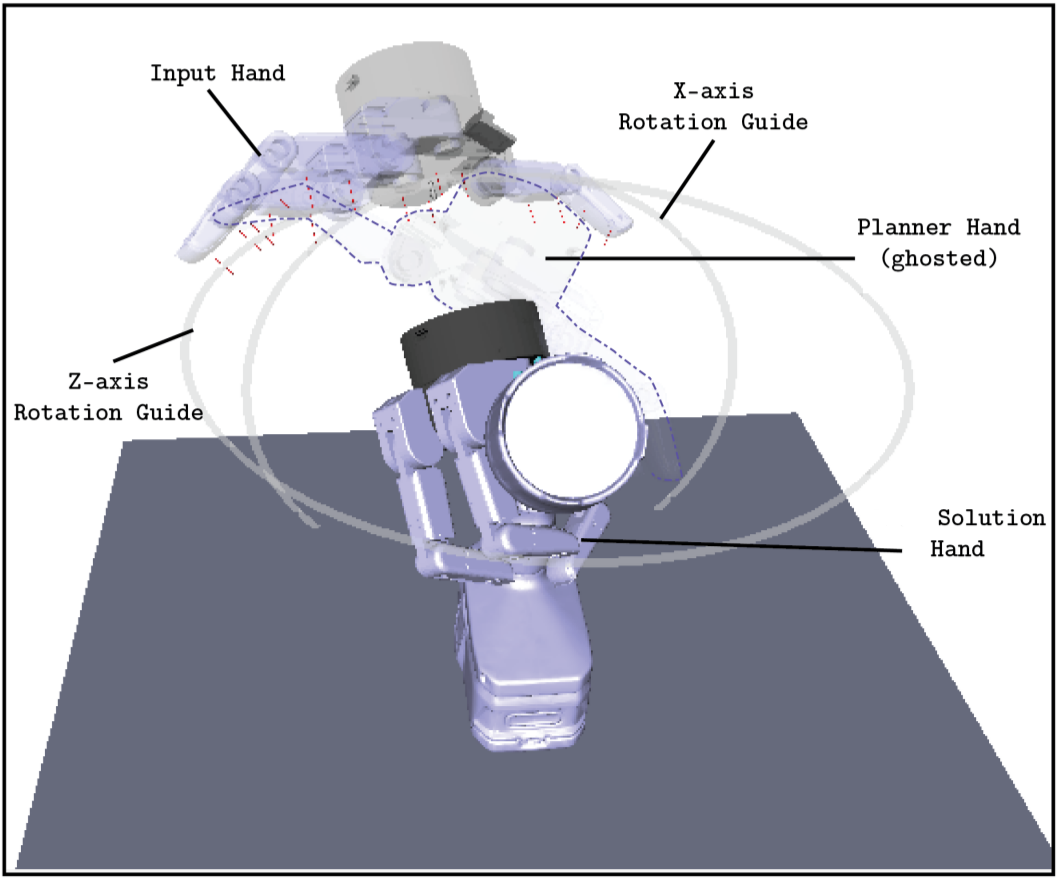
\includegraphics[width=.95\columnwidth]{ui_1.png}\\
	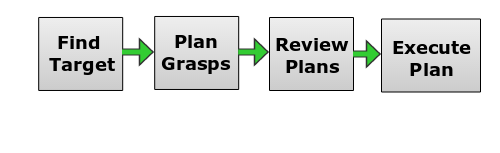
\includegraphics[width=.99\columnwidth]{images_4/overview_pipeline.png}\\
	\caption{ \emph{Top:} An annotated screenshot of the prototype grasp planning user interface in GraspIt!. During online planning, the user is presented with an augmented reality view of the target object and three renderings of the hand interacting with the scene. The \emph{Planner Hand}, which is the most transparent hand, demonstrates the current state of the planner. The \emph{Input Hand} which is of intermediate transparency, is the hand through which the user directs the planning system. Here you can see the rotational guides which allow the user to visualize their available control directions. The \emph{Solution Hand}, which is fully opaque, demonstrates the best grasp currently available. This is the grasp which is closest to the approach direction that the \emph{Input Hand} is demonstrating and which also has the best grasp quality. \emph{Bottom:} The four phases of a basic grasp planning task. Breaking the task into phases allows customization of the user interface for each phase independently to make optimal use of low input bandwidth.}
	\label{fig:overview_pipeline}
\end{figure}
\renewcommand*{\theHsection}{chX.\the\value{section}}
In \cite{Weisz2012c}, we developed a prototype BCI enabled grasping platform through which we outlined a general strategy for an online assistive grasping system. 
The grasping task can be decomposed into a four subtasks: Target object identification and localization, generation of grasp plans, picking an optimal plan, and executing the plan on the robot. Each subtask can be fulfilled by different modules which benefit from different user interaction strategies. By decomposing the tasks into explicit phases of a pipelined process, as in Figure \ref{fig:overview_pipeline}, we can optimize user's interaction for each phase to make the best use of input modalities with limited bandwidth while guiding the grasping platform. 
Although fully automated approaches for each of these subtasks have been the subject of extensive and ongoing research, integrating user input to create a shared-control environment that uses as much input as the user is able to supply is still a relatively unexplored field.

 There are many possible paradigms for integrating HRIs with a shared-control assistive robotic device. Traditional EMG and EEG setups are expensive and difficult to deploy. In this work, we wanted to explore the boundaries of what can be achieved with devices that are more practical for a real world assistive device, both in terms of convenience and cost. We experimented with two low cost devices for detecting EMG, the Emotiv Epoc (Emotiv Systems Inc., San Francisco, CA, USA) and a custom device described in Section \ref{sec:semg_hardware}. 

Putting the human in the loop when planning and executing the grasp in real-time fundamentally changes the nature of the problem as compared to a fully automated system. The key challenge becomes conveying information to the user effectively about the state of the system and then using the low bandwidth information gained from the user efficiently. This requires careful design of the interfaces provided to the user and of the control scheme for inferring intent from the user's input. Additionally, in order to present the user with reasonable grasping options, we need to extend the existing grasp stability analysis to deal with the most common problem that arises in unstructured environments, object localization errors due to sensor noise (See \cite{Weisz2012} for an analysis of the effect of sensor noise on the Eigengrasp Planner). 

\subsection{Prototype Design Components}
\subsubsection{Hardware Components}The manipulator arm for the initial prototype was composed of an industrial St\"{a}ubli TX60L robotic arm and a BarrettHand gripper. The object localization system was based on point clouds captured by a Microsoft Kinect depth camera. We sought an input device that might be representative of what could be achieved by a low cost BCI device in order to evaluate a user interface under realistic conditions of error and throughput. The Emotiv Epoc was chosen because of the convenience of its wireless form factor and relatively low cost. 

\subsubsection{EMG Input Processing}
The Emotiv Epoc comes with three built-in signal processing modalities designed to detect emotional affect, facial movement, and EEG evoked responses. Combining these classifiers, we were able to derive a training paradigm for detection of four facial gestures robustly. For details see \cite{Weisz2013}.

\subsection{User Interface}
We augmented the Eigengrasp Planner GUI in the GraspIt! simulator (\cite{Miller2004}) with a visualization of the grasp planning scene that includes a number of guides and fiducials that allow the user to guide the planner fully inside the simulator. The augmented grasp planning scene is illustrated in Figure \ref{fig:overview_pipeline}. 

The four facial gestures captured from the Epoc are treated as discrete on/off signals. We found some facial gestures, such as eyebrow raising, to be easier to maintain than others such as winking. These were assigned to control signals whose duration controlled some continuous value, such as position of the end effector along the guides. Two of the gestures are mapped to "Yes" and "No" inputs at decision points, while the remaining two control the rotation of the \emph{Input Hand} along the guides shown in Figure \ref{fig:overview_pipeline}. A video demonstrating the operation of this prototype can be found here: \url{https://youtu.be/_b5ecKbIHBQ}.

\subsection{Software Platform}

\subsubsection{Planning and Kinematics}
Planning for the motion of the arm is done in OpenRAVE using a bidirectional random tree planner in \cite{berenson-cbirrt}, and small linear motions near the object are planned using the TX60L's built-in inverse kinematics planner.

\subsubsection{Recognition System}
\label{sec:rec_system}
 We use the \emph{Model Ransac} method described in \cite{EfficientModelRansac} to identify and localize the target object in the scene. This method generates features from pairs of oriented points on the surface of the object. Prospective models are processed off-line and put into a hash table. Features are sampled from the sensor data and tested for collision in the hash table. If a sufficient number of collisions occurs with points on the same model, a variant of RANSAC is used to test the hypothesis that a set of points in the sensor data corresponds to a particular model at a particular location. This method has demonstrated good robustness and is extensible to multi-object scenes. 

\subsection{Evaluation and Shortcomings}
Using this grasping platform, the experimenters were able to develop an interface for the Eigengrasp Planner and access it through a noisy, EMG based interface. However, we found that users with less experience and patience were not able to interpret the information in the grasp planning scene. In order to run user experiments, we needed a more informative UI and some faster planning options.

\section{System 2: Adding Visual Feedback}
\setcounter{subsection}{0}
\renewcommand*{\theHsection}{chX.\the\value{section}}
After initial experiences with \emph{System 1}, we noted several shortcomings in the design of the user interface. With additional visual cues, we were able to add several features and allow non-expert users to successfully navigate the grasping pipeline. We added elements to the UI that are illustrative of the current state of the planner and the available options at each phase of the planner (see Figure \ref{fig:ui_2}). Additionally, this extended UI gives feedback about the position of localized object with respect to the sensed environment, allowing the user to interact directly with the localization system. With these modifications, we also enable the user to grasp "novel" objects that are not in the object database and use our pre-planned grasp database. 

\subsection{Handling Novel Objects}
\begin{figure}
	\centering
	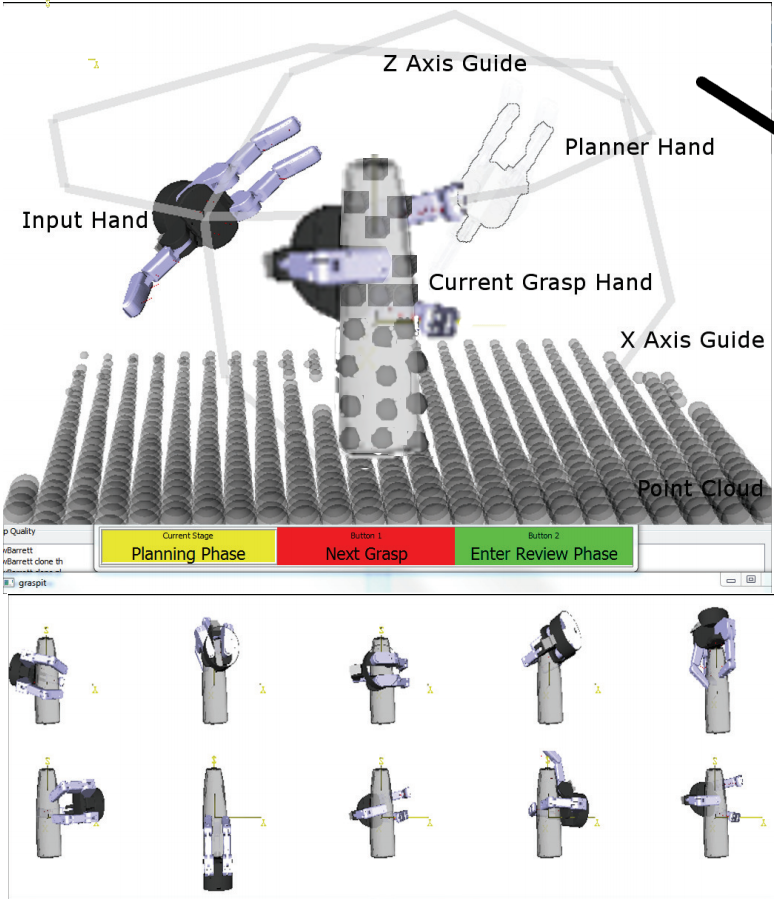
\includegraphics[width=.9\columnwidth]{ui_2_flipped.png}
	\caption{\emph{System 2 Interface - Online Planner Phase}. The user interface contains three windows: The main window containing three labeled robot hands and the target object with the aligned point cloud, the pipeline guide window containing hints for the user to guide their interaction with each phase of the planner, and the grasp view window containing rendering of the ten best grasps found by the planner thus far.}
	\label{fig:ui_2}
\end{figure}
In order to handle objects that are not in the recognition system, we rely on the stochastic nature of the planning and recognition system and the discernment of the user. When automated systems fail, the user can reject the proposed solutions and wait for another. The parameters of the object recognition system can be tuned to recognize objects with similar parts by increasing the allowed error in the hypothesis testing stage of RANSAC. An example of this alignment can be seen in Figure \ref{fig:alignment_1}. In order to allow the user to discern how well the detected object aligns to the true geometry of the novel object in the scene, the UI was modified to include a down-sampled point cloud from the depth camera. The user is responsible for rerunning the vision system until they see a reasonable alignment of the sensor data and detected model. This interaction also comes into play in the grasp planning phase, in which we rely on the user to reject grasps that may seem appropriate for the detected model but do not fit the actual unknown model well. 


\begin{figure}
\begin{subfigure}[t]{.45\columnwidth}
\centering
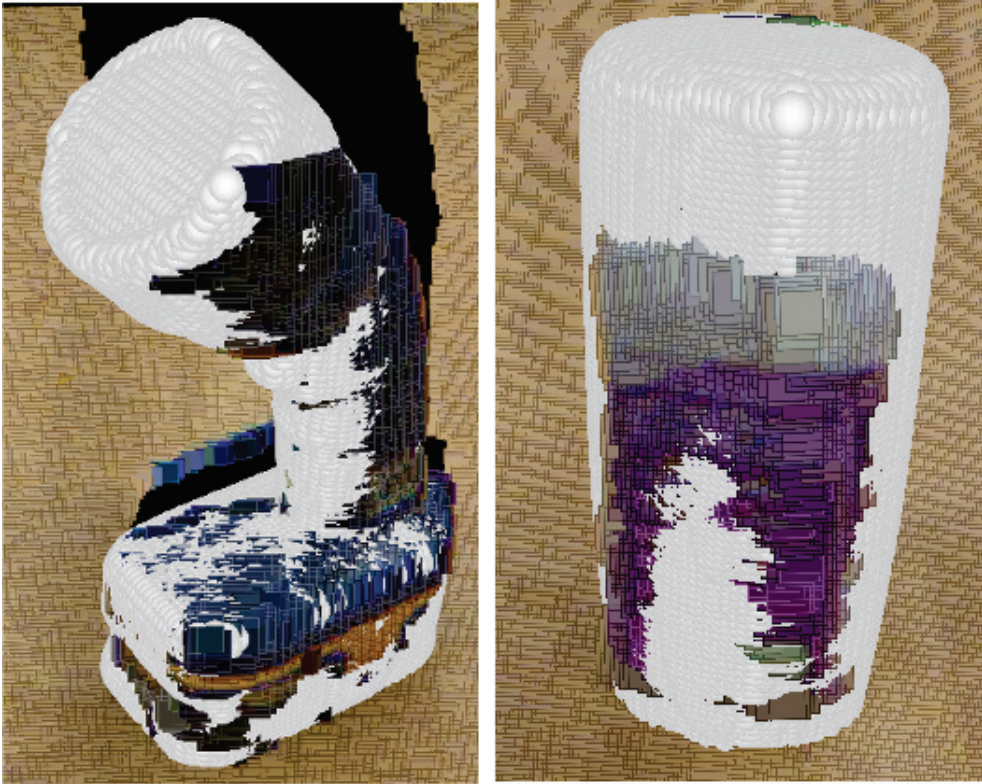
\includegraphics[height=1.2in,width=.99\columnwidth]{alignment_1.png}
\caption{Point clouds with RGB texture from the vision system. On the left is a flashlight along with its aligned point cloud in white. On the right is the point cloud of a juice bottle along with the best model from the vision system’s object database, a shampoo bottle, in white.}
\label{fig:alignment_1}
\end{subfigure}
\begin{subfigure}[t]{.45\columnwidth}
\centering
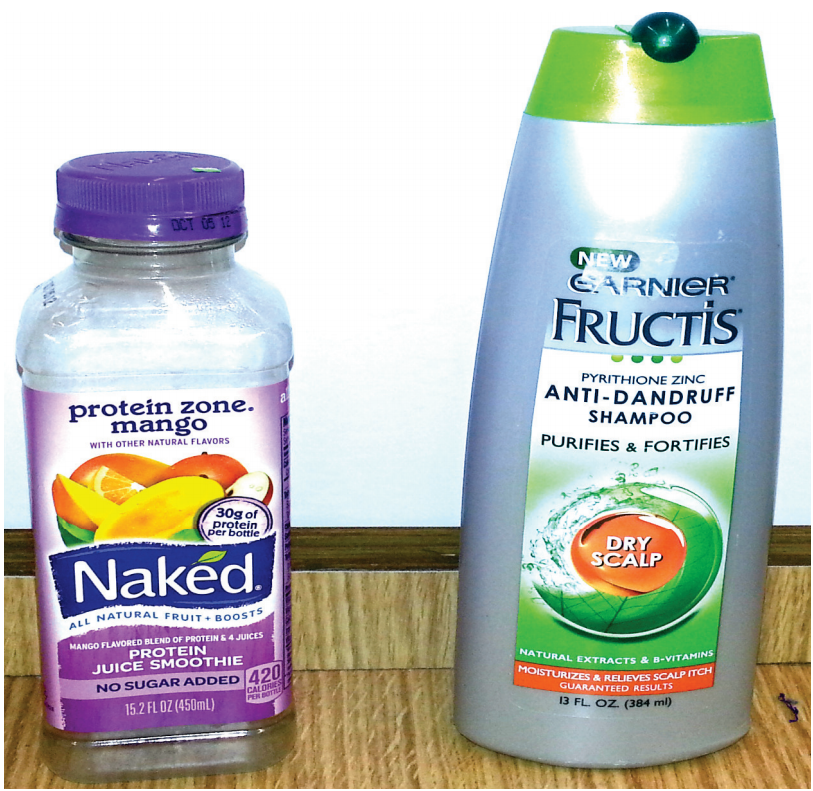
\includegraphics[height=1.2in,width=0.99\columnwidth]{unknown_objects_1.png}
\caption{The two objects which are aligned on the right of the figure above. The shampoo bottle is in the object database. The juice bottle is not. The two are roughly the same width, and this shampoo bottle can be an appropriate proxy for the juice bottle in the planner.}
\label{fig:unknown_objects_1}
\end{subfigure}
\caption{Results of the object recognition system with known and unknown objects.}
\end{figure}


\subsection{Incorporating a Grasp Database}
One useful aspect of mapping the object in the scene to a set of objects from a database is that we can also pre-plan a set of grasps for each object. This provides a method for the user to skip the slower online planning phase, since we will already rely more on the user and less on the automated grasp quality analysis. 

Using a grasp database also allows us to manually design good grasps for particular affordances that are difficult for an automated planner to recognize. Figure \ref{fig:manual_grasp_1} demonstrates such a grasp, which is realizable by the BarrettHand only because the soft plastic surface of the object deforms during grasp acquisition to allow the finger to pass through the hole in the handle region of the bottle.  In experiments, this grasp was successful 100\% of the time.  Capturing this behavior in a simulator would require modeling dynamic object deformations. Currently, accurate simulations of such properties are too slow for sampling based planners, and so human annotation of such grasps is necessary. 

To generate the grasp database, we ran the Eigengrasp Planner off-line six times for twenty minutes each with the approach direction of the palm aligned to the major axes in the positive and negative directions, using the best grasp from each direction in the database. If there were fewer than ten grasps in the database, including manually inserted grasps, then the highest quality grasps were selected from among all of the available grasps until a full ten are available. 

\subsection{Grasping Pipeline}
\begin{figure*}[ht!]
	\centering
	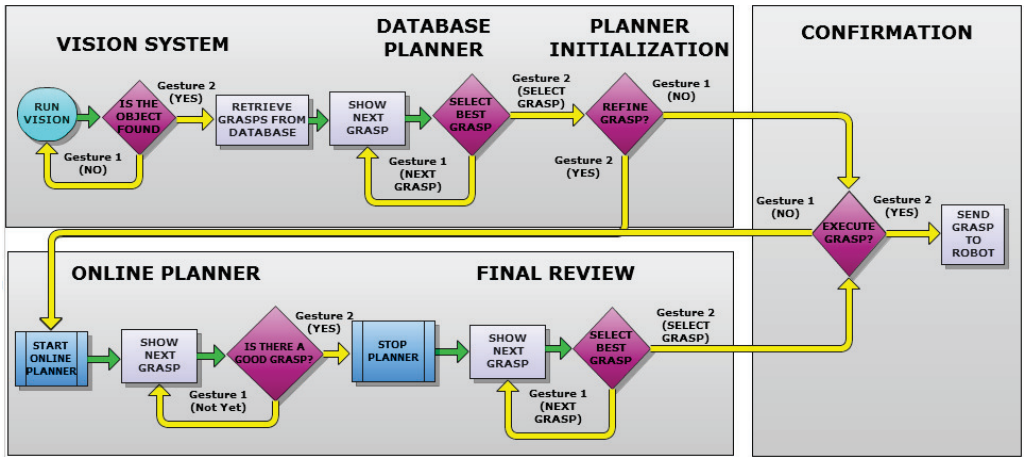
\includegraphics[width=1.7\columnwidth]{pipeline_2.png}
	\caption{The phases of the modified grasping pipeline incorporating more control over the vision system and the grasp database. If the user chooses the \emph{nth} grasp from the database, \emph{n+4} user inputs are required. If none of the grasps are suitable, the online planner can be invoked with a few simple inputs to refine one of the grasps further.}
	\label{fig:pipeline_2}
\end{figure*}
\label{sec:pipline_2}
These improvements result in a more flexible, but complex grasping pipeline. In this pipeline, there are three additional phases before the  \emph{planning-review-execute} pipeline outlined previously in which the augmented visualizations are used to provide the user with extra flexibility in initializing the planner. These phases allow the user to first control the vision systems object detection and localization, then review the set of available grasps retrieved from the pre-planned database, and finally to chose whether to activate the online refinement or simply execute the retrieved grasp. The phases of the pipeline and transitions between them are outlined as a state machine in Figure \ref{fig:pipeline_2}. Notice that these modifications create two possible paths to the final phase of grasp execution, trading off complexity for potential speed improvements. 

To help the user manage this complexity, we added a "Guide Window" that displays the transition table for the current phase, as shown in Figure \ref{fig:ui_2}. Throughout the pipeline, two of the facial gestures are associated with transitions between phases of the pipeline, while the other two provide direction to the online planner. In the "Guide Window", the left side of the window shows the current phase in yellow, the center of the window shows the result of the Gesture 1 transition in red, and the right side of the window shows the result of the Gesture 2 transition in green. 

Below the "Guide Window," we visualize the top ten grasps available to the planner. This allows the user to judge their options as they are retrieved from the database or repopulated by the online grasp planner. 


\begin{figure}
\centering
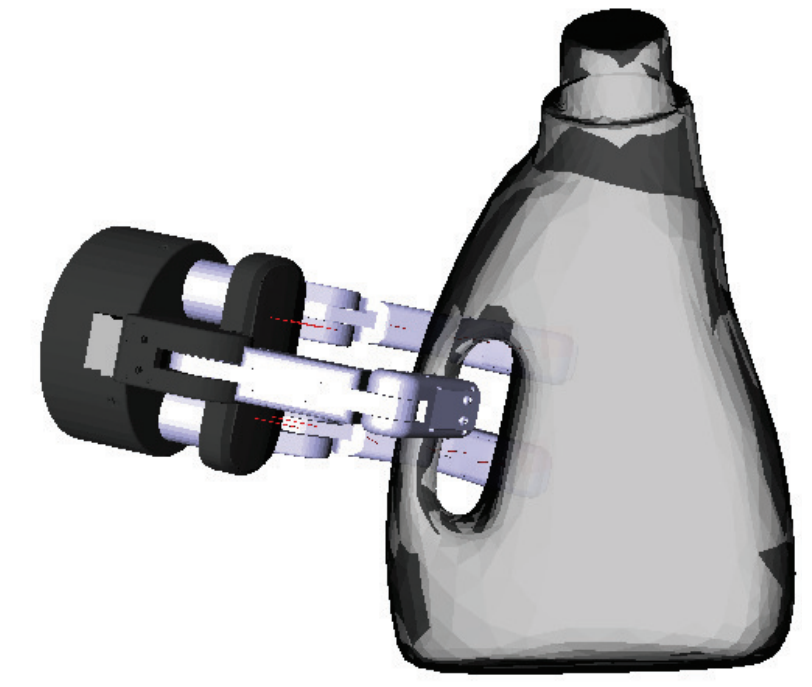
\includegraphics[height=.2\textheight]{manual_grasp_1.png}
\caption{This handle grasp for the detergent bottle is not a force closure grasp, but when chosen by the subjects in our experiments it succeeded 100\% of the time. Adding a grasp database allows such semantically relevant grasps to be used in our system.}
\label{fig:manual_grasp_1}
\end{figure}


\subsection{Experiments}
In order to test the efficacy of our system, we recruited five healthy subjects to participate in an experiment to use the system to lift three objects from a table.  All testing was approved by the Institutional Review Board of Columbia University under Protocol AAAJ6951. The results of these experiments were published in \cite{Weisz2013}, and a video illustrating the experiments can be found at \url{https://youtu.be/3YnbxVsJKs0}.

\subsubsection{Task}
Each subject was asked to grasp and lift three objects using an Emotiv Epoc as input. Two of the objects, a flashlight and a detergent bottle, were in the database and available to the vision system. One of the objects, a small juice bottle, was novel. Each subject was asked to perform two grasps, one from the top of the object and one from the side of the object. Each grasp was repeated three times. For the novel object, subjects were simply asked to grasp the object five times, irrespective of direction.


\subsubsection{Training}
\label{sec:emotiv_training}
The subject was asked to perform each facial gesture ten times each to train the Emotiv Epoc classifiers and choose reasonable parameters for the classifiers. For details, see \cite{Weisz2013} To train the subject to perform the task, the subject was asked to perform the task twice in the virtual environment without executing the final grasp on the arm. 

\subsubsection{Results}
The results of the experiments are reported in Table \ref{tab:results_2}. For each subject, we report the mean time to completion and fraction of successful attempts for each grasp. Time to completion is measured from the end of the object identification phase to the beginning of the execution phase, which is the time taken to plan the grasp. Overall, the average planning time was 104 seconds on the known objects and 86 seconds on the unknown object. The mean success rate was 80\%, demonstrating that this system is effective in allowing the user to plan and execute a reasonable grasp for these objects.
In these experiments, grasps from the side demonstrated significantly more robustness and lower planning times than grasps from above. The grasp database contained only one grasp from above for each of these objects, and this grasp was a fingertip grasp which may be sensitive to pose estimation error, which resulted in longer planning times while the subjects searched for a better grasp. In general, grasping roughly cylindrical objects such as the top of the detergent bottle from above is somewhat problematic for the BarrettHand due to its configuration and the low friction of its fingertips. In contrast, subjects were able to find a reasonable grasp from the side of the object among the grasps pulled directly from the database. The difference in planning times reflects the benefit of integrating the off-line planning phase.

\begin{table}
\centering
\begin{tabular}{ | l | c | c | c | }
\hline
Grasp & Subject & Successes & Mean Time(s) \\ \hline 
\multirow{5}{*}{Flashlight Side} & 1 & 3/3 & 125 \\ 
& 2 & 3/3 & 53 \\ 
& 3 & 2/3 & 103 \\
& 4 & 3/3 & 95 \\
& 5 & 3/3 & 82 \\ \hline
\multirow{5}{*}{Flashlight Top} & 1 & 3/3 & 132 \\ 
& 2 & 2/3 & 75 \\ 
& 3 & 2/3 & 96 \\
& 4 & 3/3 & 93 \\
& 5 & 2/3 & 125 \\ \hline
\multirow{5}{*}{\begin{minipage}{.75in}Detergent Bottle Side\end{minipage}} & 1 & 3/3 & 75 \\ 
& 2 & 3/3 & 57 \\ 
& 3 & 3/3 & 106 \\
& 4 & 2/3 & 82 \\
& 5 & 3/3 & 75 \\ \hline
\multirow{5}{*}{\begin{minipage}{.75in}Detergent Bottle Top\end{minipage}} & 1 & 1/3 & 151 \\ 
& 2 & 2/3 & 114 \\ 
& 3 & 2/3 & 142\\
& 4 & 2/3 & 161 \\
& 5 & 3/3 & 145 \\ \hline
\multirow{5}{*}{Novel Bottle} & 1 & 3/5 & 132 \\
&2 & 4/5 & 63\\
&3 & 4/5 & 95\\
&4 & 4/5 & 91\\
&5 & 4/5 & 50\\
\hline\end{tabular}
\caption{Results from Experiment 2}
\label{tab:results_2}
\end{table}

\subsection{Discussion}
During the experiment, we found that it was necessary to re-wet the electrodes of the Epoc many times during the experiment. Additionally, for three of our subjects it took more than an hour to find the right thresholds and position for the headset. After the experiment, subjects were asked to describe their discomfort during the experiment and their level of control. Subjects reported little discomfort initially, but were frustrated with the difficulty of getting the Epoc to recognize their intended actions, especially with false negatives making it difficult to continue to the next phase of the pipeline at will. This led to overemphasis of the facial gestures, which caused muscle fatigue. In spite of this frustration, subjects were able to complete the task. 

However, these difficulties pose a major problem in testing this system on a disabled subject. Since they are dependent on caretakers, an indeterminately long setup time poses a major problem in performing studies with that population. Another major source of issues is the lack of online reachability testing in the grasp planner. In these experiments, we placed the object carefully to avoid having the planner find unreachable grasps. In more cluttered scenes, this issue would be problematic. Finally, users reported that the pipeline guide window was difficult to read while focused on the task.

In the next section, we describe a different interface device that is designed specifically to measure facial EMG signals, along with some of the changes we made to the user interface to address the concerns subjects expressed during this experiment.
